% fig_gac_framework.tex — GAC Framework Pipeline
% Usage: % fig_gac_framework.tex — GAC Framework Pipeline (TikZ)
% Usage: % fig_gac_framework.tex — GAC Framework Pipeline (TikZ)
% Usage: % fig_gac_framework.tex — GAC Framework Pipeline (TikZ)
% Usage: \input{figures/fig_gac_framework.tex}
\begin{figure*}[t]
\centering
\begin{tikzpicture}[scale=0.78, every node/.style={scale=0.78},
    >=stealth,
    % Colors
    cblue/.style={fill={rgb,255:red,55;green,131;blue,187}},
    cred/.style={fill={rgb,255:red,211;green,63;blue,73}},
    cgreen/.style={fill={rgb,255:red,56;green,158;blue,92}},
    corange/.style={fill={rgb,255:red,230;green,159;blue,0}},
    cgray/.style={fill=gray!15},
    % Box styles
    phase/.style={draw, rounded corners=5pt, minimum width=2.4cm, minimum height=1.6cm,
                  line width=0.9pt, text=white, font=\sffamily\small, align=center},
    constraint/.style={draw, rounded corners=3pt, minimum width=2.0cm, minimum height=0.7cm,
                       line width=0.7pt, font=\sffamily\scriptsize, align=center,
                       fill=yellow!12, draw=orange!60!black},
    result/.style={draw, rounded corners=5pt, minimum width=2.2cm, minimum height=1.6cm,
                   line width=1.2pt, font=\sffamily\small, align=center},
    lbl/.style={font=\sffamily\small, align=center},
    arrow/.style={->, line width=1.4pt, color=gray!70!black},
    dasharrow/.style={->, line width=1.0pt, dashed, color=gray!50},
  ]

  % ===== LEFT: Analysis (§3) =====
  \node[phase, cgray, text=black, minimum width=2.0cm, minimum height=1.2cm]
    (sdpa) at (0, 1.2) {\textbf{SDPA}\\[-1pt]{\scriptsize FA2 template}\\[-1pt]{\scriptsize backend}};
  \node[phase, cgray, text=black, minimum width=2.0cm, minimum height=1.2cm]
    (gemm) at (0, -0.5) {\textbf{GEMM}\\[-1pt]{\scriptsize kernel tier}\\[-1pt]{\scriptsize heuristic}};
  \node[phase, cgray, text=black, minimum width=2.0cm, minimum height=1.2cm]
    (hw) at (0, -2.2) {\textbf{Hardware}\\[-1pt]{\scriptsize TC / VecLoad}\\[-1pt]{\scriptsize L2 (neg.)}};

  % Brace for analysis
  \node[above=0.15cm of sdpa, font=\sffamily\bfseries\small] {\S3 Analysis};
  \draw[decorate, decoration={brace, amplitude=6pt, raise=2pt}, line width=0.8pt]
    ([xshift=1.2cm]sdpa.north east) -- ([xshift=1.2cm]hw.south east);

  % ===== CENTER: Constraints =====
  \node[constraint, minimum width=3.0cm, minimum height=2.8cm]
    (constraints) at (4.0, -0.5) {};
  \node[above=-0.1cm of constraints.north, font=\sffamily\bfseries\small] {Constraints};
  \node[font=\sffamily\scriptsize, align=left, anchor=north] at ([yshift=-0.3cm]constraints.north) {
    $d \bmod 8 = 0$\\[1pt]
    $d \leq$ FA2 template\\[1pt]
    dim\%8 kernel tier\\[1pt]
    avoid cliff dims\\[1pt]
    CTA wave quant.
  };

  % Arrows: analysis → constraints
  \draw[arrow] ([xshift=1.0cm]sdpa.east) -- ([yshift=0.9cm]constraints.west);
  \draw[arrow] ([xshift=1.0cm]gemm.east) -- (constraints.west);
  \draw[arrow] ([xshift=1.0cm]hw.east) -- ([yshift=-0.9cm]constraints.west);

  % ===== RIGHT: Two paths =====
  % Path A: GAC DP (new compression)
  \node[phase, cblue, minimum width=2.6cm, minimum height=1.4cm]
    (score) at (8.0, 1.0) {\textbf{Score}\\[-1pt]{\scriptsize Fisher info}};
  \node[phase, cblue, minimum width=2.6cm, minimum height=1.4cm]
    (dp) at (11.2, 1.0) {\textbf{DP Solve}\\[-1pt]{\scriptsize knapsack}\\[-1pt]{\scriptsize align to $a$}};
  \node[phase, cblue, minimum width=2.6cm, minimum height=1.4cm]
    (svd) at (14.4, 1.0) {\textbf{SVD}\\[-1pt]{\scriptsize aligned ranks}};

  % Path B: Dimension Repair (existing model)
  \node[phase, cgreen, minimum width=2.6cm, minimum height=1.4cm]
    (detect) at (8.0, -2.0) {\textbf{Detect}\\[-1pt]{\scriptsize misaligned $d$}};
  \node[phase, cgreen, minimum width=2.6cm, minimum height=1.4cm]
    (pad) at (11.2, -2.0) {\textbf{Zero-Pad}\\[-1pt]{\scriptsize $d \to \lceil d/a\rceil \cdot a$}};
  \node[phase, cgreen, minimum width=2.6cm, minimum height=1.4cm]
    (exact) at (14.4, -2.0) {\textbf{Bit-Exact}\\[-1pt]{\scriptsize output}};

  % Arrows within paths
  \draw[arrow, color={rgb,255:red,55;green,131;blue,187}] (score) -- (dp);
  \draw[arrow, color={rgb,255:red,55;green,131;blue,187}] (dp) -- (svd);
  \draw[arrow, color={rgb,255:red,56;green,158;blue,92}] (detect) -- (pad);
  \draw[arrow, color={rgb,255:red,56;green,158;blue,92}] (pad) -- (exact);

  % Constraints → paths
  \draw[arrow] (constraints.east) -- ++(0.8,0) |- ([xshift=-0.3cm]score.west)
    node[pos=0.25, above, font=\sffamily\scriptsize\itshape] {};
  \draw[arrow] (constraints.east) -- ++(0.8,0) |- ([xshift=-0.3cm]detect.west);

  % Constraints feeds into DP
  \draw[dasharrow, color=orange!70!black]
    ([yshift=0.4cm]constraints.east) -- ++(0.8,0) |- ([yshift=0.2cm]dp.west)
    node[pos=0.82, above, font=\sffamily\scriptsize\itshape, text=orange!70!black] {candidates};

  % Path labels
  \node[above=0.15cm of dp, font=\sffamily\bfseries\small, text={rgb,255:red,55;green,131;blue,187}]
    {Path A: New Compression (\S\ref{sec:gac})};
  \node[below=0.15cm of pad, font=\sffamily\bfseries\small, text={rgb,255:red,56;green,158;blue,92}]
    {Path B: Post-Hoc Repair (\S\ref{sec:repair})};

  % Results on the right
  \node[result, fill=blue!5, draw={rgb,255:red,55;green,131;blue,187},
        right=0.6cm of svd, minimum height=1.4cm] (resA) {
    {\small\bfseries 100\% aligned}\\[-1pt]
    {\scriptsize PPL 14.30}\\[-1pt]
    {\scriptsize W.Dev 2{,}217}
  };
  \node[result, fill=green!5, draw={rgb,255:red,56;green,158;blue,92},
        right=0.6cm of exact, minimum height=1.4cm] (resB) {
    {\small\bfseries +87\% speedup}\\[-1pt]
    {\scriptsize bit-exact}\\[-1pt]
    {\scriptsize +3.7\% mem}
  };
  \draw[arrow, color={rgb,255:red,55;green,131;blue,187}] (svd) -- (resA);
  \draw[arrow, color={rgb,255:red,56;green,158;blue,92}] (exact) -- (resB);

  % Input on the left
  \node[draw, rounded corners=3pt, fill=white, line width=0.7pt,
        font=\sffamily\scriptsize, align=center, minimum width=1.8cm]
    (input) at (-3.2, -0.5) {Pre-trained\\LLM\\+ budget $B$};
  \draw[arrow] (input) -- ([xshift=-0.3cm]gemm.west |- input);

\end{tikzpicture}
\caption{\textbf{GAC framework overview.}
Analysis (\S\ref{sec:analysis}) extracts alignment constraints from three layers (SDPA, GEMM, hardware).
These constraints drive two complementary solutions:
\emph{Path~A}---alignment-aware rank allocation via multi-choice knapsack DP for new compression;
\emph{Path~B}---zero-padding repair for already-compressed models.
Both paths produce fully-aligned dimensions with no accuracy loss (DP) or bit-exact output preservation (repair).}
\label{fig:gac_framework}
\end{figure*}

\begin{figure*}[t]
\centering
\begin{tikzpicture}[scale=0.78, every node/.style={scale=0.78},
    >=stealth,
    % Colors
    cblue/.style={fill={rgb,255:red,55;green,131;blue,187}},
    cred/.style={fill={rgb,255:red,211;green,63;blue,73}},
    cgreen/.style={fill={rgb,255:red,56;green,158;blue,92}},
    corange/.style={fill={rgb,255:red,230;green,159;blue,0}},
    cgray/.style={fill=gray!15},
    % Box styles
    phase/.style={draw, rounded corners=5pt, minimum width=2.4cm, minimum height=1.6cm,
                  line width=0.9pt, text=white, font=\sffamily\small, align=center},
    constraint/.style={draw, rounded corners=3pt, minimum width=2.0cm, minimum height=0.7cm,
                       line width=0.7pt, font=\sffamily\scriptsize, align=center,
                       fill=yellow!12, draw=orange!60!black},
    result/.style={draw, rounded corners=5pt, minimum width=2.2cm, minimum height=1.6cm,
                   line width=1.2pt, font=\sffamily\small, align=center},
    lbl/.style={font=\sffamily\small, align=center},
    arrow/.style={->, line width=1.4pt, color=gray!70!black},
    dasharrow/.style={->, line width=1.0pt, dashed, color=gray!50},
  ]

  % ===== LEFT: Analysis (§3) =====
  \node[phase, cgray, text=black, minimum width=2.0cm, minimum height=1.2cm]
    (sdpa) at (0, 1.2) {\textbf{SDPA}\\[-1pt]{\scriptsize FA2 template}\\[-1pt]{\scriptsize backend}};
  \node[phase, cgray, text=black, minimum width=2.0cm, minimum height=1.2cm]
    (gemm) at (0, -0.5) {\textbf{GEMM}\\[-1pt]{\scriptsize kernel tier}\\[-1pt]{\scriptsize heuristic}};
  \node[phase, cgray, text=black, minimum width=2.0cm, minimum height=1.2cm]
    (hw) at (0, -2.2) {\textbf{Hardware}\\[-1pt]{\scriptsize TC / VecLoad}\\[-1pt]{\scriptsize L2 (neg.)}};

  % Brace for analysis
  \node[above=0.15cm of sdpa, font=\sffamily\bfseries\small] {\S3 Analysis};
  \draw[decorate, decoration={brace, amplitude=6pt, raise=2pt}, line width=0.8pt]
    ([xshift=1.2cm]sdpa.north east) -- ([xshift=1.2cm]hw.south east);

  % ===== CENTER: Constraints =====
  \node[constraint, minimum width=3.0cm, minimum height=2.8cm]
    (constraints) at (4.0, -0.5) {};
  \node[above=-0.1cm of constraints.north, font=\sffamily\bfseries\small] {Constraints};
  \node[font=\sffamily\scriptsize, align=left, anchor=north] at ([yshift=-0.3cm]constraints.north) {
    $d \bmod 8 = 0$\\[1pt]
    $d \leq$ FA2 template\\[1pt]
    dim\%8 kernel tier\\[1pt]
    avoid cliff dims\\[1pt]
    CTA wave quant.
  };

  % Arrows: analysis → constraints
  \draw[arrow] ([xshift=1.0cm]sdpa.east) -- ([yshift=0.9cm]constraints.west);
  \draw[arrow] ([xshift=1.0cm]gemm.east) -- (constraints.west);
  \draw[arrow] ([xshift=1.0cm]hw.east) -- ([yshift=-0.9cm]constraints.west);

  % ===== RIGHT: Two paths =====
  % Path A: GAC DP (new compression)
  \node[phase, cblue, minimum width=2.6cm, minimum height=1.4cm]
    (score) at (8.0, 1.0) {\textbf{Score}\\[-1pt]{\scriptsize Fisher info}};
  \node[phase, cblue, minimum width=2.6cm, minimum height=1.4cm]
    (dp) at (11.2, 1.0) {\textbf{DP Solve}\\[-1pt]{\scriptsize knapsack}\\[-1pt]{\scriptsize align to $a$}};
  \node[phase, cblue, minimum width=2.6cm, minimum height=1.4cm]
    (svd) at (14.4, 1.0) {\textbf{SVD}\\[-1pt]{\scriptsize aligned ranks}};

  % Path B: Dimension Repair (existing model)
  \node[phase, cgreen, minimum width=2.6cm, minimum height=1.4cm]
    (detect) at (8.0, -2.0) {\textbf{Detect}\\[-1pt]{\scriptsize misaligned $d$}};
  \node[phase, cgreen, minimum width=2.6cm, minimum height=1.4cm]
    (pad) at (11.2, -2.0) {\textbf{Zero-Pad}\\[-1pt]{\scriptsize $d \to \lceil d/a\rceil \cdot a$}};
  \node[phase, cgreen, minimum width=2.6cm, minimum height=1.4cm]
    (exact) at (14.4, -2.0) {\textbf{Bit-Exact}\\[-1pt]{\scriptsize output}};

  % Arrows within paths
  \draw[arrow, color={rgb,255:red,55;green,131;blue,187}] (score) -- (dp);
  \draw[arrow, color={rgb,255:red,55;green,131;blue,187}] (dp) -- (svd);
  \draw[arrow, color={rgb,255:red,56;green,158;blue,92}] (detect) -- (pad);
  \draw[arrow, color={rgb,255:red,56;green,158;blue,92}] (pad) -- (exact);

  % Constraints → paths
  \draw[arrow] (constraints.east) -- ++(0.8,0) |- ([xshift=-0.3cm]score.west)
    node[pos=0.25, above, font=\sffamily\scriptsize\itshape] {};
  \draw[arrow] (constraints.east) -- ++(0.8,0) |- ([xshift=-0.3cm]detect.west);

  % Constraints feeds into DP
  \draw[dasharrow, color=orange!70!black]
    ([yshift=0.4cm]constraints.east) -- ++(0.8,0) |- ([yshift=0.2cm]dp.west)
    node[pos=0.82, above, font=\sffamily\scriptsize\itshape, text=orange!70!black] {candidates};

  % Path labels
  \node[above=0.15cm of dp, font=\sffamily\bfseries\small, text={rgb,255:red,55;green,131;blue,187}]
    {Path A: New Compression (\S\ref{sec:gac})};
  \node[below=0.15cm of pad, font=\sffamily\bfseries\small, text={rgb,255:red,56;green,158;blue,92}]
    {Path B: Post-Hoc Repair (\S\ref{sec:repair})};

  % Results on the right
  \node[result, fill=blue!5, draw={rgb,255:red,55;green,131;blue,187},
        right=0.6cm of svd, minimum height=1.4cm] (resA) {
    {\small\bfseries 100\% aligned}\\[-1pt]
    {\scriptsize PPL 14.30}\\[-1pt]
    {\scriptsize W.Dev 2{,}217}
  };
  \node[result, fill=green!5, draw={rgb,255:red,56;green,158;blue,92},
        right=0.6cm of exact, minimum height=1.4cm] (resB) {
    {\small\bfseries +87\% speedup}\\[-1pt]
    {\scriptsize bit-exact}\\[-1pt]
    {\scriptsize +3.7\% mem}
  };
  \draw[arrow, color={rgb,255:red,55;green,131;blue,187}] (svd) -- (resA);
  \draw[arrow, color={rgb,255:red,56;green,158;blue,92}] (exact) -- (resB);

  % Input on the left
  \node[draw, rounded corners=3pt, fill=white, line width=0.7pt,
        font=\sffamily\scriptsize, align=center, minimum width=1.8cm]
    (input) at (-3.2, -0.5) {Pre-trained\\LLM\\+ budget $B$};
  \draw[arrow] (input) -- ([xshift=-0.3cm]gemm.west |- input);

\end{tikzpicture}
\caption{\textbf{GAC framework overview.}
Analysis (\S\ref{sec:analysis}) extracts alignment constraints from three layers (SDPA, GEMM, hardware).
These constraints drive two complementary solutions:
\emph{Path~A}---alignment-aware rank allocation via multi-choice knapsack DP for new compression;
\emph{Path~B}---zero-padding repair for already-compressed models.
Both paths produce fully-aligned dimensions with no accuracy loss (DP) or bit-exact output preservation (repair).}
\label{fig:gac_framework}
\end{figure*}

\begin{figure*}[t]
\centering
\begin{tikzpicture}[scale=0.78, every node/.style={scale=0.78},
    >=stealth,
    % Colors
    cblue/.style={fill={rgb,255:red,55;green,131;blue,187}},
    cred/.style={fill={rgb,255:red,211;green,63;blue,73}},
    cgreen/.style={fill={rgb,255:red,56;green,158;blue,92}},
    corange/.style={fill={rgb,255:red,230;green,159;blue,0}},
    cgray/.style={fill=gray!15},
    % Box styles
    phase/.style={draw, rounded corners=5pt, minimum width=2.4cm, minimum height=1.6cm,
                  line width=0.9pt, text=white, font=\sffamily\small, align=center},
    constraint/.style={draw, rounded corners=3pt, minimum width=2.0cm, minimum height=0.7cm,
                       line width=0.7pt, font=\sffamily\scriptsize, align=center,
                       fill=yellow!12, draw=orange!60!black},
    result/.style={draw, rounded corners=5pt, minimum width=2.2cm, minimum height=1.6cm,
                   line width=1.2pt, font=\sffamily\small, align=center},
    lbl/.style={font=\sffamily\small, align=center},
    arrow/.style={->, line width=1.4pt, color=gray!70!black},
    dasharrow/.style={->, line width=1.0pt, dashed, color=gray!50},
  ]

  % ===== LEFT: Analysis (§3) =====
  \node[phase, cgray, text=black, minimum width=2.0cm, minimum height=1.2cm]
    (sdpa) at (0, 1.2) {\textbf{SDPA}\\[-1pt]{\scriptsize FA2 template}\\[-1pt]{\scriptsize backend}};
  \node[phase, cgray, text=black, minimum width=2.0cm, minimum height=1.2cm]
    (gemm) at (0, -0.5) {\textbf{GEMM}\\[-1pt]{\scriptsize kernel tier}\\[-1pt]{\scriptsize heuristic}};
  \node[phase, cgray, text=black, minimum width=2.0cm, minimum height=1.2cm]
    (hw) at (0, -2.2) {\textbf{Hardware}\\[-1pt]{\scriptsize TC / VecLoad}\\[-1pt]{\scriptsize L2 (neg.)}};

  % Brace for analysis
  \node[above=0.15cm of sdpa, font=\sffamily\bfseries\small] {\S3 Analysis};
  \draw[decorate, decoration={brace, amplitude=6pt, raise=2pt}, line width=0.8pt]
    ([xshift=1.2cm]sdpa.north east) -- ([xshift=1.2cm]hw.south east);

  % ===== CENTER: Constraints =====
  \node[constraint, minimum width=3.0cm, minimum height=2.8cm]
    (constraints) at (4.0, -0.5) {};
  \node[above=-0.1cm of constraints.north, font=\sffamily\bfseries\small] {Constraints};
  \node[font=\sffamily\scriptsize, align=left, anchor=north] at ([yshift=-0.3cm]constraints.north) {
    $d \bmod 8 = 0$\\[1pt]
    $d \leq$ FA2 template\\[1pt]
    dim\%8 kernel tier\\[1pt]
    avoid cliff dims\\[1pt]
    CTA wave quant.
  };

  % Arrows: analysis → constraints
  \draw[arrow] ([xshift=1.0cm]sdpa.east) -- ([yshift=0.9cm]constraints.west);
  \draw[arrow] ([xshift=1.0cm]gemm.east) -- (constraints.west);
  \draw[arrow] ([xshift=1.0cm]hw.east) -- ([yshift=-0.9cm]constraints.west);

  % ===== RIGHT: Two paths =====
  % Path A: GAC DP (new compression)
  \node[phase, cblue, minimum width=2.6cm, minimum height=1.4cm]
    (score) at (8.0, 1.0) {\textbf{Score}\\[-1pt]{\scriptsize Fisher info}};
  \node[phase, cblue, minimum width=2.6cm, minimum height=1.4cm]
    (dp) at (11.2, 1.0) {\textbf{DP Solve}\\[-1pt]{\scriptsize knapsack}\\[-1pt]{\scriptsize align to $a$}};
  \node[phase, cblue, minimum width=2.6cm, minimum height=1.4cm]
    (svd) at (14.4, 1.0) {\textbf{SVD}\\[-1pt]{\scriptsize aligned ranks}};

  % Path B: Dimension Repair (existing model)
  \node[phase, cgreen, minimum width=2.6cm, minimum height=1.4cm]
    (detect) at (8.0, -2.0) {\textbf{Detect}\\[-1pt]{\scriptsize misaligned $d$}};
  \node[phase, cgreen, minimum width=2.6cm, minimum height=1.4cm]
    (pad) at (11.2, -2.0) {\textbf{Zero-Pad}\\[-1pt]{\scriptsize $d \to \lceil d/a\rceil \cdot a$}};
  \node[phase, cgreen, minimum width=2.6cm, minimum height=1.4cm]
    (exact) at (14.4, -2.0) {\textbf{Bit-Exact}\\[-1pt]{\scriptsize output}};

  % Arrows within paths
  \draw[arrow, color={rgb,255:red,55;green,131;blue,187}] (score) -- (dp);
  \draw[arrow, color={rgb,255:red,55;green,131;blue,187}] (dp) -- (svd);
  \draw[arrow, color={rgb,255:red,56;green,158;blue,92}] (detect) -- (pad);
  \draw[arrow, color={rgb,255:red,56;green,158;blue,92}] (pad) -- (exact);

  % Constraints → paths
  \draw[arrow] (constraints.east) -- ++(0.8,0) |- ([xshift=-0.3cm]score.west)
    node[pos=0.25, above, font=\sffamily\scriptsize\itshape] {};
  \draw[arrow] (constraints.east) -- ++(0.8,0) |- ([xshift=-0.3cm]detect.west);

  % Constraints feeds into DP
  \draw[dasharrow, color=orange!70!black]
    ([yshift=0.4cm]constraints.east) -- ++(0.8,0) |- ([yshift=0.2cm]dp.west)
    node[pos=0.82, above, font=\sffamily\scriptsize\itshape, text=orange!70!black] {candidates};

  % Path labels
  \node[above=0.15cm of dp, font=\sffamily\bfseries\small, text={rgb,255:red,55;green,131;blue,187}]
    {Path A: New Compression (\S\ref{sec:gac})};
  \node[below=0.15cm of pad, font=\sffamily\bfseries\small, text={rgb,255:red,56;green,158;blue,92}]
    {Path B: Post-Hoc Repair (\S\ref{sec:repair})};

  % Results on the right
  \node[result, fill=blue!5, draw={rgb,255:red,55;green,131;blue,187},
        right=0.6cm of svd, minimum height=1.4cm] (resA) {
    {\small\bfseries 100\% aligned}\\[-1pt]
    {\scriptsize PPL 14.30}\\[-1pt]
    {\scriptsize W.Dev 2{,}217}
  };
  \node[result, fill=green!5, draw={rgb,255:red,56;green,158;blue,92},
        right=0.6cm of exact, minimum height=1.4cm] (resB) {
    {\small\bfseries +87\% speedup}\\[-1pt]
    {\scriptsize bit-exact}\\[-1pt]
    {\scriptsize +3.7\% mem}
  };
  \draw[arrow, color={rgb,255:red,55;green,131;blue,187}] (svd) -- (resA);
  \draw[arrow, color={rgb,255:red,56;green,158;blue,92}] (exact) -- (resB);

  % Input on the left
  \node[draw, rounded corners=3pt, fill=white, line width=0.7pt,
        font=\sffamily\scriptsize, align=center, minimum width=1.8cm]
    (input) at (-3.2, -0.5) {Pre-trained\\LLM\\+ budget $B$};
  \draw[arrow] (input) -- ([xshift=-0.3cm]gemm.west |- input);

\end{tikzpicture}
\caption{\textbf{GAC framework overview.}
Analysis (\S\ref{sec:analysis}) extracts alignment constraints from three layers (SDPA, GEMM, hardware).
These constraints drive two complementary solutions:
\emph{Path~A}---alignment-aware rank allocation via multi-choice knapsack DP for new compression;
\emph{Path~B}---zero-padding repair for already-compressed models.
Both paths produce fully-aligned dimensions with no accuracy loss (DP) or bit-exact output preservation (repair).}
\label{fig:gac_framework}
\end{figure*}

\begin{figure*}[t]
\centering
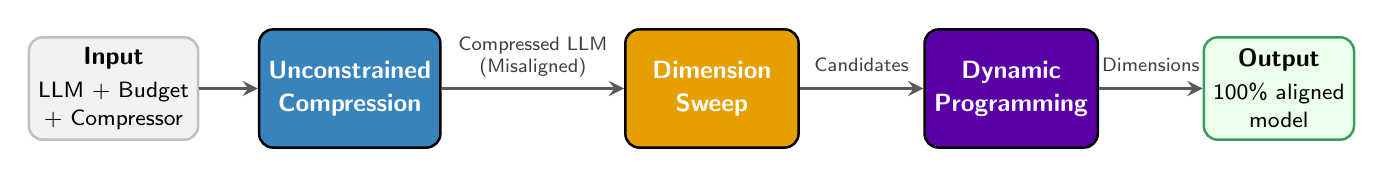
\begin{tikzpicture}[scale=1.0, every node/.style={scale=1.0},
    >=stealth,
    % Colors
    cblue/.style={fill={rgb,255:red,55;green,131;blue,187}},
    cred/.style={fill={rgb,255:red,211;green,63;blue,73}},
    cgreen/.style={fill={rgb,255:red,56;green,158;blue,92}},
    corange/.style={fill={rgb,255:red,230;green,159;blue,0}},
    % Styles
    phase/.style={draw, rounded corners=5pt, minimum width=2.2cm, minimum height=1.5cm,
                  line width=0.9pt, font=\sffamily\small, align=center},
    iobox/.style={draw, rounded corners=5pt, minimum width=1.8cm, minimum height=1.3cm,
                  line width=0.9pt, font=\sffamily\small, align=center},
    arrow/.style={->, line width=1.4pt, color=gray!70!black},
    lbl/.style={font=\sffamily\scriptsize, align=center, text=gray!50!black},
  ]

  % Input
  \node[iobox, fill=gray!10, draw=gray!50] (input) at (0, 0) {
    \textbf{Input}\\[1pt]
    {\footnotesize LLM + Budget}\\[-1pt]
    {\footnotesize + Compressor}
  };

  % Step 1: Unconstrained Compression
  \node[phase, cblue, text=white] (compress) at (3.0, 0) {
    \textbf{Unconstrained}\\[1pt]
    \textbf{Compression}
  };

  % Step 2: Dimension Sweep
  \node[phase, corange, text=white] (sweep) at (7.6, 0) {
    \textbf{Dimension}\\[1pt]
    \textbf{Sweep}
  };

  % Step 3: Knapsack DP
  \node[phase, fill=violet!70!blue, text=white] (dp) at (11.4, 0) {
    \textbf{Dynamic}\\[1pt]
    \textbf{Programming}
  };

  % Output
  \node[iobox, fill=green!8, draw={rgb,255:red,56;green,158;blue,92}] (output) at (14.8, 0) {
    \textbf{Output}\\[1pt]
    {\footnotesize 100\% aligned}\\[-1pt]
    {\footnotesize model}
  };

  % Arrows
  \draw[arrow] (input) -- (compress);
  \draw[arrow] (compress) -- (sweep) node[midway, above=0pt, lbl] {Compressed LLM\\(Misaligned)};
  \draw[arrow] (sweep) -- (dp) node[midway, above=2pt, lbl] {Candidates};
  \draw[arrow] (dp) -- (output) node[midway, above=2pt, lbl] {Dimensions};

\end{tikzpicture}
\caption{GAC pipeline: compress → sweep → optimize → aligned model.}
\label{fig:gac_framework}
\end{figure*}
